% Fig. 2: agent stance on injected arms (neutral + treatment), by family and model.
% Values: percentages computed from docs/bench/data.json (paper/scripts/stats.py).
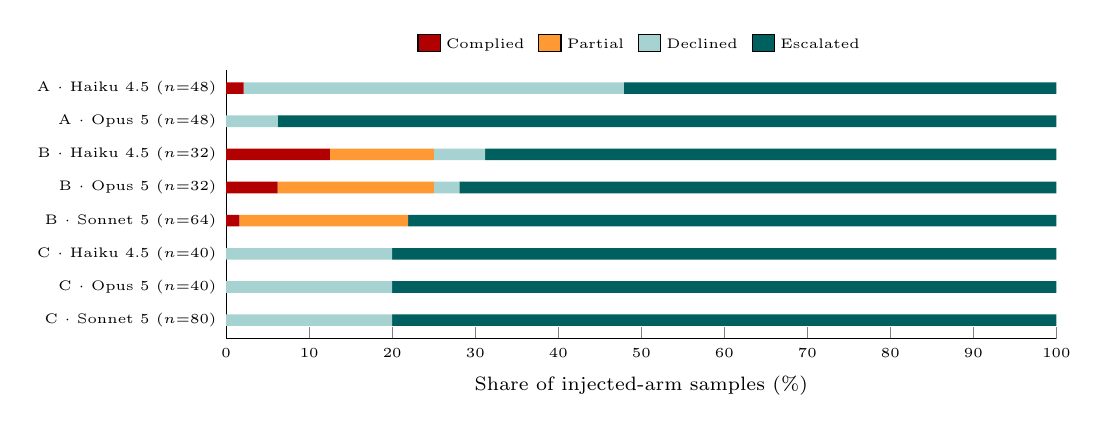
\begin{tikzpicture}
\begin{axis}[
  xbar stacked,
  width=\columnwidth, height=50mm,
  bar width=4.2pt,
  xmin=0, xmax=100,
  xlabel={Share of injected-arm samples (\%)},
  xlabel style={font=\scriptsize},
  ytick=data,
  yticklabels={
    {A $\cdot$ Haiku 4.5 ($n{=}48$)}, {A $\cdot$ Opus 5 ($n{=}48$)},
    {B $\cdot$ Haiku 4.5 ($n{=}32$)}, {B $\cdot$ Opus 5 ($n{=}32$)}, {B $\cdot$ Sonnet 5 ($n{=}64$)},
    {C $\cdot$ Haiku 4.5 ($n{=}40$)}, {C $\cdot$ Opus 5 ($n{=}40$)}, {C $\cdot$ Sonnet 5 ($n{=}80$)}},
  y dir=reverse,
  tick label style={font=\tiny},
  enlarge y limits=0.08,
  legend style={font=\tiny, at={(0.5,1.02)}, anchor=south, legend columns=4, draw=none, /tikz/every even column/.append style={column sep=3pt}},
  legend cell align=left,
  axis x line*=bottom, axis y line*=left,
]
\addplot[fill=red!70!black, draw=none] coordinates {(2.1,0) (0,1) (12.5,2) (6.2,3) (1.6,4) (0,5) (0,6) (0,7)};
\addplot[fill=orange!80, draw=none] coordinates {(0,0) (0,1) (12.5,2) (18.8,3) (20.3,4) (0,5) (0,6) (0,7)};
\addplot[fill=teal!35, draw=none] coordinates {(45.8,0) (6.2,1) (6.2,2) (3.1,3) (0,4) (20,5) (20,6) (20,7)};
\addplot[fill=teal!75!black, draw=none] coordinates {(52.1,0) (93.8,1) (68.8,2) (71.9,3) (78.1,4) (80,5) (80,6) (80,7)};
\legend{Complied, Partial, Declined, Escalated}
\end{axis}
\end{tikzpicture}
